 
 \begin{figure}[htbp]
	\centering
		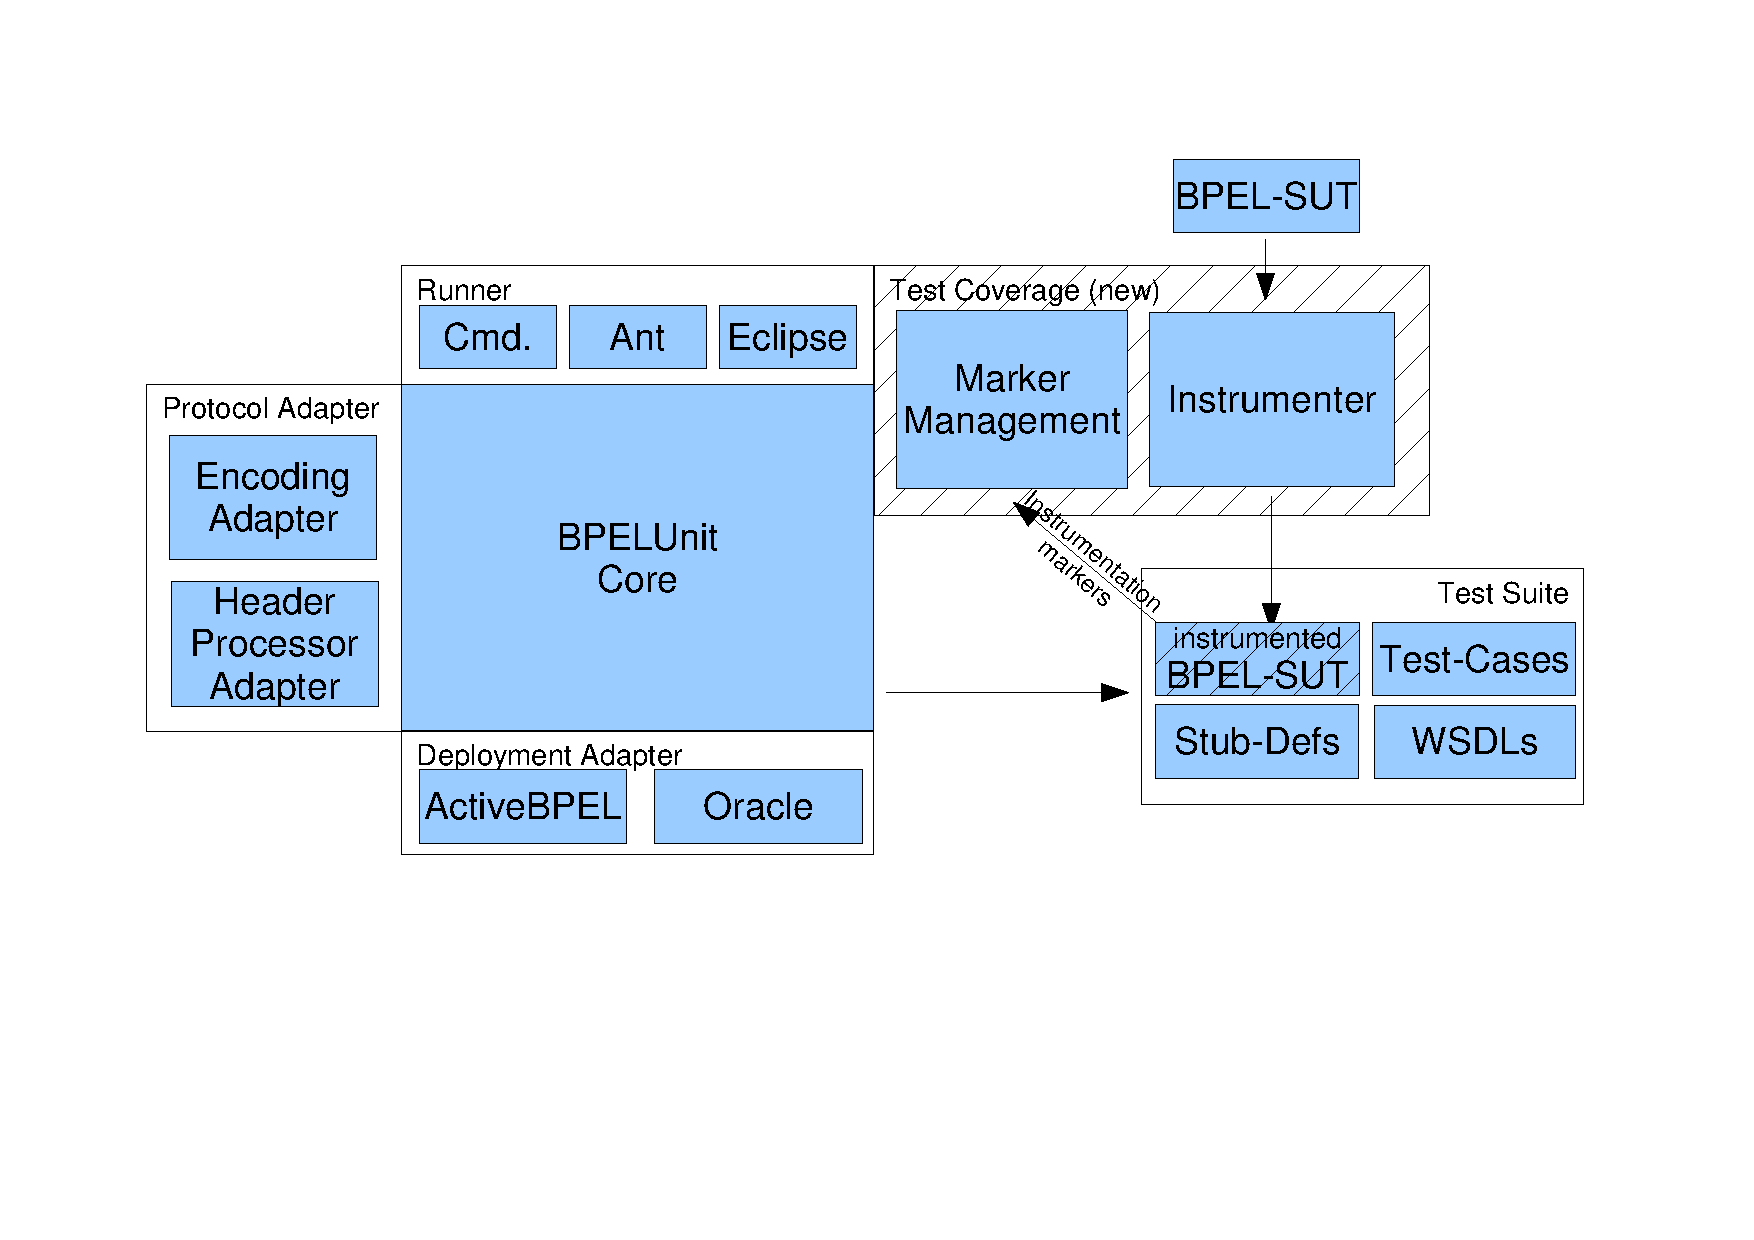
\includegraphics[width=0.9\textwidth]{bilder/bpelunit-architecture-with-coverage.pdf}
		\caption{Kontrollfluss eines BPEL Prozesses}
	\label{fig:ExamlpleBPELProzess}
\end{figure}

BPELUnit Framework wird erweitert durch hinzuf�gen einer Phase vor dem tats�chlichen Testen. In dieser Phase wird der BPEL Prozess annotiert , invoke-Aktivit�ten werdenhnzugef�gt. Diese Aktivit�teb sind Markierungen f�r jede Aktivit�t und jede M�glichkeit des Kontrollflusses. Die Marken haben eindeutige Identifizierungen, die verwendet werden umd die Relation zwischen Marken und Aktivit�ten bzw. dem Kontrollflu� 

Zur Laufzeit diese Aktivit��ten rufen ein Web Service des BPELUnit Frameworks . Bei diesen Aufrufen werden die Marken transportiert. , die signalisieren den Asf�hrungspfad zum BPELUnit Framework. Diesse Marken werden auf den BPEL Prozess abgebildet. Nach der Ausf�hrung k�nnen mit Hilfe der Marken und statischen Informationen �ber BPEL Prozess die Abdeckungsmetriken berechnet werden. Es ist ein neuer Modul hinzugekommen, der alle Aufgaben, die mit der Messung der Abdeckung zu tun haben, managt. So enth�lt dieser Modul einen Instrumentierer der den BPEL file analysiert und Annotationen hinzuf�gt. Der alte File wird durch den neuen ersetzt.  Zus�tzlich ist ein Web Service f�r das Empfangen von Marken in diesem Modul enhalten